\documentclass[a4paper]{article}

\usepackage{INTERSPEECH2021}

% Put the lab number of the corresponding exercise
\title{Language Modelling - Lab 4}
\name{Marco Prosperi (257857)}

\address{
  University of Trento}
\email{marco.prosperi@studenti.unitn.it}

\begin{document}

\maketitle
%
%Dear students, \\
%here you can find a complete description of the sections that you need to write for the mini-report. You have to write a mini-report of \textbf{max 1 page (references, tables and images are excluded from the count)} for each last exercise of labs 4 (LM) and 5 (NLU). \textbf{Reports longer than 1 page will not be checked.} The purpose of this is to give you a way to report cleanly the results and give you space to describe what you have done and/or the originality that you have added to the exercise.
%\\
%\textbf{If you did part A only, you have to just report the results in a table with a small description.}
%
\section{Introduction}
The first part of the project aimed to improve the baseline RNN performance by incrementally adding 
features and dynamically adjusting hyperparameters (learning rate, hidden units,
embedding size). The model was trained on the Penn Treebank dataset, using perplexity
as the main evaluation metric. In the second part, advanced techniques \cite{merityRegOpt} were 
incorporated to further enhance the language model, including Weight Tying 
to reduce parameters, Variational Dropout (excluding DropConnect) for 
regularization, and Averaged Stochastic Gradient Descent (AvSGD) for better
optimization. These improvements aimed to enhance generalization and 
convergence while maintaining low perplexity (less than 250). 

\section{Implementation details}

The first part of the project involved implementing a basic RNN model using PyTorch, 
based on the code provided by the teaching assistant in the Lab Repository \cite{nlu-labs-unitn}.
 I started by integrating the functions, model, and dataset from the Jupyter notebook into my own 
 repository. Initially, the RNN model was trained on the Penn Treebank dataset, yielding a high 
 perplexity that did not meet the target of 250. To address this, I experimented with various 
 hyperparameters, including the learning rate, hidden units, and embedding size, eventually 
 achieving an acceptable perplexity. Subsequently, I developed an LSTM model, which significantly 
 lowered the perplexity to 137.31. To further enhance performance, I incorporated two dropout layers,
  resulting in better model accuracy. Additionally, the adoption of AdamW, a weight decay optimizer, 
  further reduced the perplexity to 105.46. Given the consistent performance improvements, I retained
   these regularization techniques for the second part of the project.


In the second phase, I focused on implementing advanced techniques
 to further optimize the language model. The first enhancement was Weight Tying,
  which decreased the model’s parameter count and improved generalization. I also 
  introduced Variational Dropout \cite{gal2016theoreticallygroundedapplicationdropout}, 
  a method specifically designed for recurrent neural networks that applies a fixed dropout 
  mask across the entire input sequence, enhancing temporal consistency and training stability.

Finally, I employed the Non-monotonically triggered AvSGD \cite{merityRegOpt}, which 
switches to AvSGD when SGD converges to a steady-state distribution. The technique can be
 activated when model performance plateaus, as recommended by the authors: AvSGD is initiated 
 when the validation metric does not improve over multiple cycles. A practical implementation 
 involves using a patience mechanism similar to early stopping; once patience is exhausted, AvSGD
  is triggered, and patience is reset to enable early termination. Alternatively, the switch 
  can occur when validation loss exceeds the minimum observed within a non-monotonic window, a 
  strategy inspired by the official Salesforce Research repository \cite{salesforce-repo}.

\section{Results}
The results of my experiments are summarized in Table \ref{tab:results}.

In the first phase of the project, I started with a basic RNN model and experimented with different hyperparameters. 
After some tuning, the model achieved a perplexity of 173.22. Subsequently, I implemented several techniques that contributed 
to improved performance in each step. The validation perplexity is shown in Figure \ref{fig:plot}, which illustrates the results 
of the LSTM model with dropout layers and AdamW optimizer.

\begin{figure}[h!]
\centering
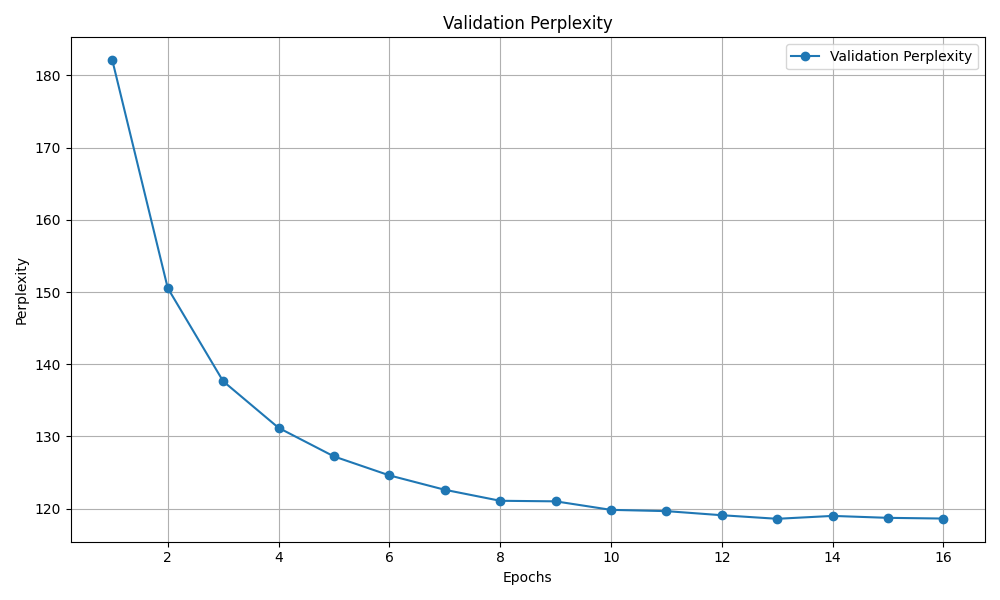
\includegraphics[width=0.8\linewidth]{images/part_A.png}
\caption{Validation perplexity of the LSTM model with dropout layers and AdamW.}
\label{fig:plot}
\end{figure}

In the second phase, I focused on implementing advanced optimization techniques, building upon
 the best model from the previous step. This improved model achieved a perplexity of 90.56, with
  a learning rate of 2, and both hidden and embedding units set to 400. One important observation
   was that the performance of the model improved when using a learning rate scheduler that decreased
    the learning rate over time, rather than relying on a fixed learning rate. Specifically, I used 
    a StepLR scheduler with a step size of 5 and a gamma of 0.75.

    Additionally, I observed that when AvSGD was triggered, the training loss increased 
    temporarily. This behavior stems from the shift in optimization dynamics: when switching
    
    from standard SGD to AvSGD, the model begins averaging past parameter updates, which can 
    disrupt the immediate optimization trajectory. While this averaging improves long-term 
    stability and generalization, it may initially raise the training loss as the model adapts
     to the new update regime.

    Furthermore, the learning rate scheduler (StepLR) compounds this effect—when the learning 
    rate is reduced, the model’s updates become more conservative, requiring additional steps 
    to re-stabilize convergence. The temporary loss increase reflects this adjustment period, 
    where the model transitions toward a flatter, and often more generalizable, minimum in the
     loss landscape.

     \begin{figure}[h!]
      \centering
      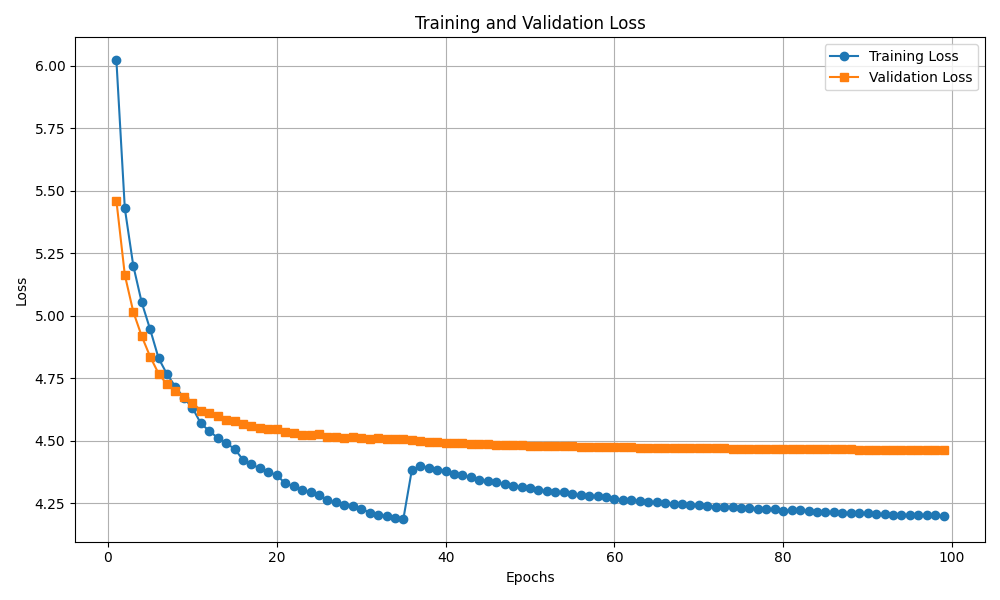
\includegraphics[width=0.8\linewidth]{images/part_A_avsdg.png}
      \caption{Trigger point of AvSGD}
      \label{fig:plot-avsdg}
      \end{figure}
\newpage



\begin{table}[h!]
  \centering
  \begin{tabular}{l p{1 cm} p{1 cm} p{1 cm} p{1 cm}}
      \midrule
      \textbf{Model} & \textbf{PPL} & \textbf{LR} & \textbf{Hidden} & \textbf{Emb} \\
      \midrule
      \multicolumn{5}{c}{\textbf{Part A}} \\
      RNN                     & 173.22 & 0.1    & 100 & 100 \\
      LSTM                    & 137.31 & 2      & 300 & 300 \\
      LSTM + Dropout Layers      & 123.14 & 2      & 300 & 300 \\
      LSTM + Dropout Layers + AdamW & 105.46 & 0.001 & 250 & 300 \\
      \midrule
      \multicolumn{5}{c}{\textbf{Part B}} \\
      \midrule
      LSTM + Weight Tying + Var Dropout + AvSDG & 90.56 & 2 & 400 & 400 \\
      \bottomrule
  \end{tabular}
  \caption{Perplexity and hyperparameters of the best models.}
  \label{tab:results}
\end{table}


\bibliographystyle{IEEEtran}

\bibliography{mybib}

\end{document}
